% fig:shortcuts_overview -- conceptual taxonomy of non-identity shortcut traits.
% Single-column TikZ (design width 8.2 cm = \columnwidth), native-size fonts,
% no \resizebox, no node-nested \tikz, no \newcommand-pics. Schematic glyphs
% only, no real-face imagery. Suggested include (figure env + caption live in
% main.tex):
%   \begin{figure}[t]\centering% fig:shortcuts_overview -- conceptual taxonomy of non-identity shortcut traits.
% Single-column TikZ (design width 8.2 cm = \columnwidth), native-size fonts,
% no \resizebox, no node-nested \tikz, no \newcommand-pics. Schematic glyphs
% only, no real-face imagery. Suggested include (figure env + caption live in
% main.tex):
%   \begin{figure}[t]\centering% fig:shortcuts_overview -- conceptual taxonomy of non-identity shortcut traits.
% Single-column TikZ (design width 8.2 cm = \columnwidth), native-size fonts,
% no \resizebox, no node-nested \tikz, no \newcommand-pics. Schematic glyphs
% only, no real-face imagery. Suggested include (figure env + caption live in
% main.tex):
%   \begin{figure}[t]\centering% fig:shortcuts_overview -- conceptual taxonomy of non-identity shortcut traits.
% Single-column TikZ (design width 8.2 cm = \columnwidth), native-size fonts,
% no \resizebox, no node-nested \tikz, no \newcommand-pics. Schematic glyphs
% only, no real-face imagery. Suggested include (figure env + caption live in
% main.tex):
%   \begin{figure}[t]\centering\input{figures/shortcuts_overview.tex}...\end{figure}
% Verdicts are the registered reads from results.tex; do not paraphrase stronger.
\centering
\definecolor{tzBlue}{RGB}{47,76,166}
\definecolor{tzOrange}{RGB}{214,116,34}
\definecolor{tzGray}{RGB}{95,100,110}
\definecolor{tzDark}{RGB}{45,50,60}
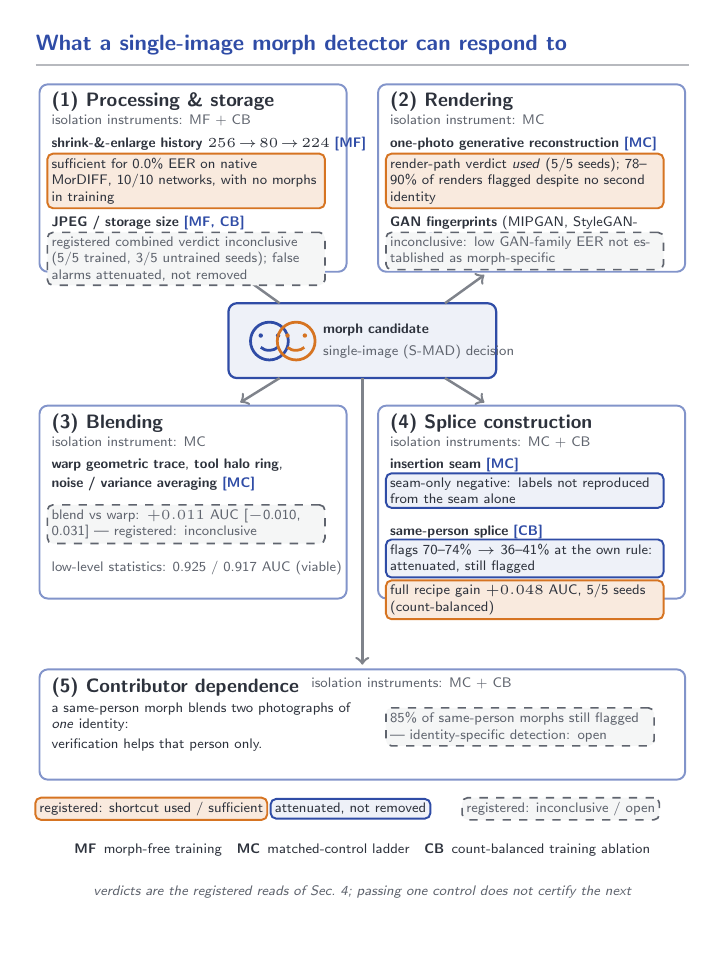
\begin{tikzpicture}[
  x=1cm,y=1cm,
  font=\sffamily,
  every node/.style={align=left, inner sep=1.5pt, outer sep=0pt},
  fline/.style={line width=1.0pt},
  hrule/.style={draw=tzGray!45, line width=0.6pt},
  boxR/.style={draw=tzBlue, fill=tzBlue!8, rounded corners=3pt, line width=0.8pt},
  fam/.style={draw=tzBlue!60, fill=white, rounded corners=3pt, line width=0.7pt},
  head/.style={anchor=west, font=\sffamily\bfseries\footnotesize, text=tzBlue},
  famHead/.style={anchor=north west, font=\sffamily\bfseries\scriptsize, text=tzDark},
  sub/.style={anchor=north west, font=\sffamily\tiny, text=tzGray},
  trait/.style={anchor=north west, font=\sffamily\tiny, text=tzDark},
  vEst/.style={draw=tzOrange, fill=tzOrange!15, rounded corners=2pt, line width=0.7pt,
               font=\sffamily\tiny, text=tzDark},
  vAtt/.style={draw=tzBlue, fill=tzBlue!8, rounded corners=2pt, line width=0.7pt,
               font=\sffamily\tiny, text=tzDark},
  vInc/.style={draw=tzGray, dashed, fill=tzGray!6, rounded corners=2pt, line width=0.6pt,
               font=\sffamily\tiny, text=tzGray},
  hint/.style={anchor=north west, font=\sffamily\tiny, text=tzGray},
  spoke/.style={->, tzGray!80, line width=0.9pt},
  qlab/.style={font=\sffamily\tiny\itshape, text=tzGray},
]
\useasboundingbox (-0.15,0.05) rectangle (8.35,11.50);

% ============================================================== header
\node[head] at (-0.1,11.28) {What a single-image morph detector can respond to};
\draw[hrule] (-0.05,11.03) -- (8.25,11.03);

% ============================================================== hub node
\draw[boxR] (2.40,7.05) rectangle (5.80,8.00);
\begin{scope}[shift={(3.02,7.52)}]
  \draw[fline, tzBlue] (-0.10,0) circle (0.24);
  \fill[tzBlue] (-0.21,0.07) circle (0.028);
  \fill[tzBlue] (0.01,0.07) circle (0.028);
  \draw[fline, tzBlue] (-0.21,-0.08) arc (215:325:0.13 and 0.09);
  \draw[fline, tzOrange] (0.24,0) circle (0.24);
  \fill[tzOrange] (0.13,0.07) circle (0.028);
  \fill[tzOrange] (0.35,0.07) circle (0.028);
  \draw[fline, tzOrange] (0.13,-0.08) arc (215:325:0.13 and 0.09);
\end{scope}
\node[anchor=west, font=\sffamily\tiny\bfseries, text=tzDark] at (3.55,7.66)
  {morph candidate};
\node[anchor=west, font=\sffamily\tiny, text=tzGray] at (3.55,7.38)
  {single-image (S-MAD) decision};

% ------------------------------------- radiating spokes: hub to trait groups
% top-left
\draw[spoke] (3.05,8.00) -- (2.55,8.36);
% top-right
\draw[spoke] (5.15,8.00) -- (5.65,8.36);
% bottom-left
\draw[spoke] (3.05,7.05) -- (2.55,6.74);
% bottom-right
\draw[spoke] (5.15,7.05) -- (5.65,6.74);
% center: down the corridor between the lower boxes to (5) contributor
\draw[spoke] (4.10,7.05) -- (4.10,3.41);

% ================================================================ 1 TL
\draw[fam] (0.00,8.40) rectangle (3.90,10.78);
\node[famHead] at (0.10,10.73) {(1) Processing \& storage};
\node[sub] at (0.10,10.44) {isolation instruments: MF + CB};
\node[trait] at (0.10,10.16)
  {\textbf{shrink-\&-enlarge history} $256\!\to\!80\!\to\!224$ {\color{tzBlue}\textbf{[MF]}}};
\node[vEst, anchor=north west, text width=3.42cm] at (0.10,9.90)
  {sufficient for 0.0\% EER on native MorDIFF, 10/10 networks, with no morphs in training};
\node[trait] at (0.10,9.16) {\textbf{JPEG / storage size} {\color{tzBlue}\textbf{[MF, CB]}}};
\node[vInc, anchor=north west, text width=3.42cm] at (0.10,8.90)
  {registered combined verdict inconclusive (5/5 trained, 3/5 untrained seeds); false alarms attenuated, not removed};

% ================================================================ 2 TR
\draw[fam] (4.30,8.40) rectangle (8.20,10.78);
\node[famHead] at (4.40,10.73) {(2) Rendering};
\node[sub] at (4.40,10.44) {isolation instrument: MC};
\node[trait] at (4.40,10.16)
  {\textbf{one-photo generative reconstruction} {\color{tzBlue}\textbf{[MC]}}};
\node[vEst, anchor=north west, text width=3.42cm] at (4.40,9.90)
  {render-path verdict \emph{used} (5/5 seeds); 78--90\% of renders flagged despite no second identity};
\node[trait, text width=3.42cm] at (4.40,9.16)
  {\textbf{GAN fingerprints} (MIPGAN, StyleGAN-style) {\color{tzBlue}\textbf{[MC]}}};
\node[vInc, anchor=north west, text width=3.42cm] at (4.40,8.90)
  {inconclusive: low GAN-family EER not established as morph-specific};

% ================================================================ 3 BL
\draw[fam] (0.00,4.25) rectangle (3.90,6.70);
\node[famHead] at (0.10,6.65) {(3) Blending};
\node[sub] at (0.10,6.36) {isolation instrument: MC};
\node[trait, text width=3.42cm] at (0.10,6.08)
  {\textbf{warp geometric trace}, \textbf{tool halo ring},\\[1pt]
   \textbf{noise / variance averaging} {\color{tzBlue}\textbf{[MC]}}};
\node[vInc, anchor=north west, text width=3.42cm] at (0.10,5.44)
  {blend vs warp: $+0.011$ AUC [$-$0.010, 0.031] --- registered: inconclusive};
\node[hint] at (0.10,4.78)
  {low-level statistics: 0.925 / 0.917 AUC (viable)};

% ================================================================ 4 BR
\draw[fam] (4.30,4.25) rectangle (8.20,6.70);
\node[famHead] at (4.40,6.65) {(4) Splice construction};
\node[sub] at (4.40,6.36) {isolation instruments: MC + CB};
\node[trait] at (4.40,6.08) {\textbf{insertion seam} {\color{tzBlue}\textbf{[MC]}}};
\node[vAtt, anchor=north west, text width=3.42cm] at (4.40,5.84)
  {seam-only negative: labels not reproduced from the seam alone};
\node[trait] at (4.40,5.24) {\textbf{same-person splice} {\color{tzBlue}\textbf{[CB]}}};
\node[vAtt, anchor=north west, text width=3.42cm] at (4.40,5.00)
  {flags 70--74\% $\to$ 36--41\% at the own rule: attenuated, still flagged};
\node[vEst, anchor=north west, text width=3.42cm] at (4.40,4.48)
  {full recipe gain $+0.048$ AUC, 5/5 seeds (count-balanced)};

% ================================================================ 5 band
\draw[fam] (0.00,1.95) rectangle (8.20,3.35);
\node[famHead] at (0.10,3.30) {(5) Contributor dependence};
\node[sub] at (3.40,3.30) {isolation instruments: MC + CB};
\node[trait, text width=3.95cm] at (0.10,2.98)
  {a same-person morph blends two photographs of \emph{one} identity:\\[1pt]
   verification helps that person only.};
\node[vInc, anchor=west, text width=3.30cm] at (4.40,2.62)
  {85\% of same-person morphs still flagged --- identity-specific detection: open};

% ============================================================== legend
\node[vEst] at (1.42,1.58) {registered: shortcut used / sufficient};
\node[vAtt] at (3.95,1.58) {attenuated, not removed};
\node[vInc] at (6.62,1.58) {registered: inconclusive / open};
\node[font=\sffamily\tiny, text=tzDark] at (4.10,1.06)
  {\textbf{MF}\, morph-free training\quad
   \textbf{MC}\, matched-control ladder\quad
   \textbf{CB}\, count-balanced training ablation};
\node[qlab] at (4.10,0.52)
  {verdicts are the registered reads of Sec.~4; passing one control does not certify the next};

\end{tikzpicture}
...\end{figure}
% Verdicts are the registered reads from results.tex; do not paraphrase stronger.
\centering
\definecolor{tzBlue}{RGB}{47,76,166}
\definecolor{tzOrange}{RGB}{214,116,34}
\definecolor{tzGray}{RGB}{95,100,110}
\definecolor{tzDark}{RGB}{45,50,60}
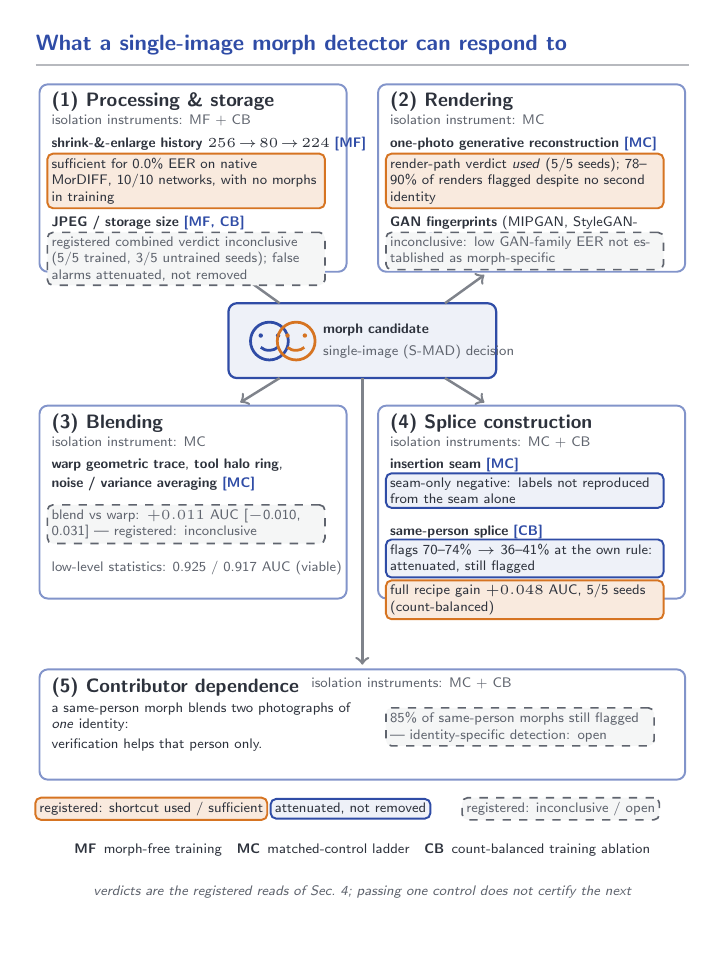
\begin{tikzpicture}[
  x=1cm,y=1cm,
  font=\sffamily,
  every node/.style={align=left, inner sep=1.5pt, outer sep=0pt},
  fline/.style={line width=1.0pt},
  hrule/.style={draw=tzGray!45, line width=0.6pt},
  boxR/.style={draw=tzBlue, fill=tzBlue!8, rounded corners=3pt, line width=0.8pt},
  fam/.style={draw=tzBlue!60, fill=white, rounded corners=3pt, line width=0.7pt},
  head/.style={anchor=west, font=\sffamily\bfseries\footnotesize, text=tzBlue},
  famHead/.style={anchor=north west, font=\sffamily\bfseries\scriptsize, text=tzDark},
  sub/.style={anchor=north west, font=\sffamily\tiny, text=tzGray},
  trait/.style={anchor=north west, font=\sffamily\tiny, text=tzDark},
  vEst/.style={draw=tzOrange, fill=tzOrange!15, rounded corners=2pt, line width=0.7pt,
               font=\sffamily\tiny, text=tzDark},
  vAtt/.style={draw=tzBlue, fill=tzBlue!8, rounded corners=2pt, line width=0.7pt,
               font=\sffamily\tiny, text=tzDark},
  vInc/.style={draw=tzGray, dashed, fill=tzGray!6, rounded corners=2pt, line width=0.6pt,
               font=\sffamily\tiny, text=tzGray},
  hint/.style={anchor=north west, font=\sffamily\tiny, text=tzGray},
  spoke/.style={->, tzGray!80, line width=0.9pt},
  qlab/.style={font=\sffamily\tiny\itshape, text=tzGray},
]
\useasboundingbox (-0.15,0.05) rectangle (8.35,11.50);

% ============================================================== header
\node[head] at (-0.1,11.28) {What a single-image morph detector can respond to};
\draw[hrule] (-0.05,11.03) -- (8.25,11.03);

% ============================================================== hub node
\draw[boxR] (2.40,7.05) rectangle (5.80,8.00);
\begin{scope}[shift={(3.02,7.52)}]
  \draw[fline, tzBlue] (-0.10,0) circle (0.24);
  \fill[tzBlue] (-0.21,0.07) circle (0.028);
  \fill[tzBlue] (0.01,0.07) circle (0.028);
  \draw[fline, tzBlue] (-0.21,-0.08) arc (215:325:0.13 and 0.09);
  \draw[fline, tzOrange] (0.24,0) circle (0.24);
  \fill[tzOrange] (0.13,0.07) circle (0.028);
  \fill[tzOrange] (0.35,0.07) circle (0.028);
  \draw[fline, tzOrange] (0.13,-0.08) arc (215:325:0.13 and 0.09);
\end{scope}
\node[anchor=west, font=\sffamily\tiny\bfseries, text=tzDark] at (3.55,7.66)
  {morph candidate};
\node[anchor=west, font=\sffamily\tiny, text=tzGray] at (3.55,7.38)
  {single-image (S-MAD) decision};

% ------------------------------------- radiating spokes: hub to trait groups
% top-left
\draw[spoke] (3.05,8.00) -- (2.55,8.36);
% top-right
\draw[spoke] (5.15,8.00) -- (5.65,8.36);
% bottom-left
\draw[spoke] (3.05,7.05) -- (2.55,6.74);
% bottom-right
\draw[spoke] (5.15,7.05) -- (5.65,6.74);
% center: down the corridor between the lower boxes to (5) contributor
\draw[spoke] (4.10,7.05) -- (4.10,3.41);

% ================================================================ 1 TL
\draw[fam] (0.00,8.40) rectangle (3.90,10.78);
\node[famHead] at (0.10,10.73) {(1) Processing \& storage};
\node[sub] at (0.10,10.44) {isolation instruments: MF + CB};
\node[trait] at (0.10,10.16)
  {\textbf{shrink-\&-enlarge history} $256\!\to\!80\!\to\!224$ {\color{tzBlue}\textbf{[MF]}}};
\node[vEst, anchor=north west, text width=3.42cm] at (0.10,9.90)
  {sufficient for 0.0\% EER on native MorDIFF, 10/10 networks, with no morphs in training};
\node[trait] at (0.10,9.16) {\textbf{JPEG / storage size} {\color{tzBlue}\textbf{[MF, CB]}}};
\node[vInc, anchor=north west, text width=3.42cm] at (0.10,8.90)
  {registered combined verdict inconclusive (5/5 trained, 3/5 untrained seeds); false alarms attenuated, not removed};

% ================================================================ 2 TR
\draw[fam] (4.30,8.40) rectangle (8.20,10.78);
\node[famHead] at (4.40,10.73) {(2) Rendering};
\node[sub] at (4.40,10.44) {isolation instrument: MC};
\node[trait] at (4.40,10.16)
  {\textbf{one-photo generative reconstruction} {\color{tzBlue}\textbf{[MC]}}};
\node[vEst, anchor=north west, text width=3.42cm] at (4.40,9.90)
  {render-path verdict \emph{used} (5/5 seeds); 78--90\% of renders flagged despite no second identity};
\node[trait, text width=3.42cm] at (4.40,9.16)
  {\textbf{GAN fingerprints} (MIPGAN, StyleGAN-style) {\color{tzBlue}\textbf{[MC]}}};
\node[vInc, anchor=north west, text width=3.42cm] at (4.40,8.90)
  {inconclusive: low GAN-family EER not established as morph-specific};

% ================================================================ 3 BL
\draw[fam] (0.00,4.25) rectangle (3.90,6.70);
\node[famHead] at (0.10,6.65) {(3) Blending};
\node[sub] at (0.10,6.36) {isolation instrument: MC};
\node[trait, text width=3.42cm] at (0.10,6.08)
  {\textbf{warp geometric trace}, \textbf{tool halo ring},\\[1pt]
   \textbf{noise / variance averaging} {\color{tzBlue}\textbf{[MC]}}};
\node[vInc, anchor=north west, text width=3.42cm] at (0.10,5.44)
  {blend vs warp: $+0.011$ AUC [$-$0.010, 0.031] --- registered: inconclusive};
\node[hint] at (0.10,4.78)
  {low-level statistics: 0.925 / 0.917 AUC (viable)};

% ================================================================ 4 BR
\draw[fam] (4.30,4.25) rectangle (8.20,6.70);
\node[famHead] at (4.40,6.65) {(4) Splice construction};
\node[sub] at (4.40,6.36) {isolation instruments: MC + CB};
\node[trait] at (4.40,6.08) {\textbf{insertion seam} {\color{tzBlue}\textbf{[MC]}}};
\node[vAtt, anchor=north west, text width=3.42cm] at (4.40,5.84)
  {seam-only negative: labels not reproduced from the seam alone};
\node[trait] at (4.40,5.24) {\textbf{same-person splice} {\color{tzBlue}\textbf{[CB]}}};
\node[vAtt, anchor=north west, text width=3.42cm] at (4.40,5.00)
  {flags 70--74\% $\to$ 36--41\% at the own rule: attenuated, still flagged};
\node[vEst, anchor=north west, text width=3.42cm] at (4.40,4.48)
  {full recipe gain $+0.048$ AUC, 5/5 seeds (count-balanced)};

% ================================================================ 5 band
\draw[fam] (0.00,1.95) rectangle (8.20,3.35);
\node[famHead] at (0.10,3.30) {(5) Contributor dependence};
\node[sub] at (3.40,3.30) {isolation instruments: MC + CB};
\node[trait, text width=3.95cm] at (0.10,2.98)
  {a same-person morph blends two photographs of \emph{one} identity:\\[1pt]
   verification helps that person only.};
\node[vInc, anchor=west, text width=3.30cm] at (4.40,2.62)
  {85\% of same-person morphs still flagged --- identity-specific detection: open};

% ============================================================== legend
\node[vEst] at (1.42,1.58) {registered: shortcut used / sufficient};
\node[vAtt] at (3.95,1.58) {attenuated, not removed};
\node[vInc] at (6.62,1.58) {registered: inconclusive / open};
\node[font=\sffamily\tiny, text=tzDark] at (4.10,1.06)
  {\textbf{MF}\, morph-free training\quad
   \textbf{MC}\, matched-control ladder\quad
   \textbf{CB}\, count-balanced training ablation};
\node[qlab] at (4.10,0.52)
  {verdicts are the registered reads of Sec.~4; passing one control does not certify the next};

\end{tikzpicture}
...\end{figure}
% Verdicts are the registered reads from results.tex; do not paraphrase stronger.
\centering
\definecolor{tzBlue}{RGB}{47,76,166}
\definecolor{tzOrange}{RGB}{214,116,34}
\definecolor{tzGray}{RGB}{95,100,110}
\definecolor{tzDark}{RGB}{45,50,60}
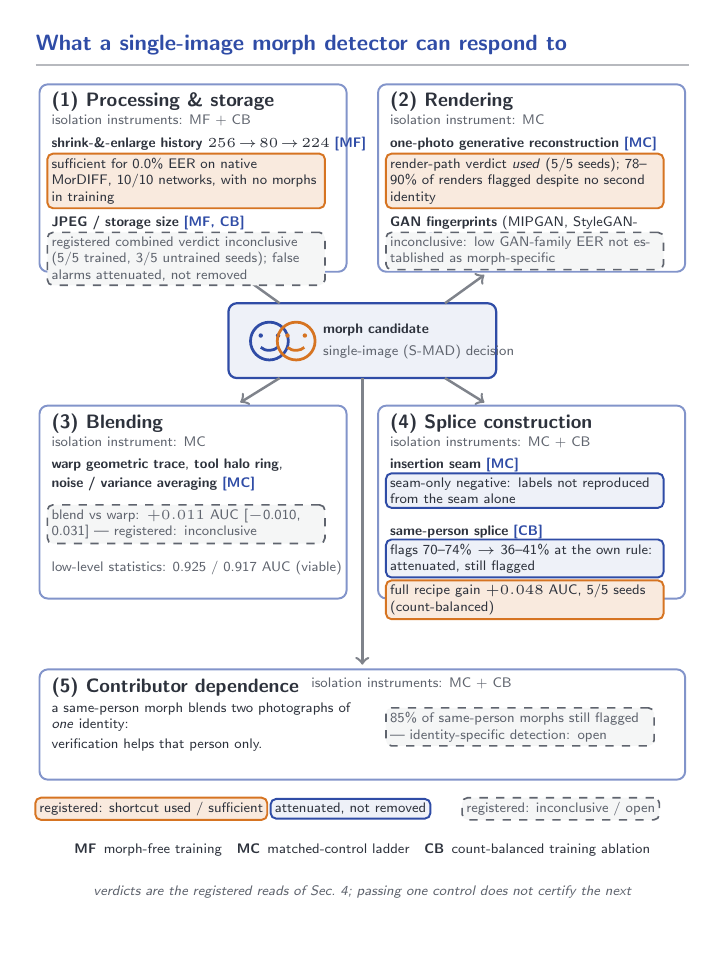
\begin{tikzpicture}[
  x=1cm,y=1cm,
  font=\sffamily,
  every node/.style={align=left, inner sep=1.5pt, outer sep=0pt},
  fline/.style={line width=1.0pt},
  hrule/.style={draw=tzGray!45, line width=0.6pt},
  boxR/.style={draw=tzBlue, fill=tzBlue!8, rounded corners=3pt, line width=0.8pt},
  fam/.style={draw=tzBlue!60, fill=white, rounded corners=3pt, line width=0.7pt},
  head/.style={anchor=west, font=\sffamily\bfseries\footnotesize, text=tzBlue},
  famHead/.style={anchor=north west, font=\sffamily\bfseries\scriptsize, text=tzDark},
  sub/.style={anchor=north west, font=\sffamily\tiny, text=tzGray},
  trait/.style={anchor=north west, font=\sffamily\tiny, text=tzDark},
  vEst/.style={draw=tzOrange, fill=tzOrange!15, rounded corners=2pt, line width=0.7pt,
               font=\sffamily\tiny, text=tzDark},
  vAtt/.style={draw=tzBlue, fill=tzBlue!8, rounded corners=2pt, line width=0.7pt,
               font=\sffamily\tiny, text=tzDark},
  vInc/.style={draw=tzGray, dashed, fill=tzGray!6, rounded corners=2pt, line width=0.6pt,
               font=\sffamily\tiny, text=tzGray},
  hint/.style={anchor=north west, font=\sffamily\tiny, text=tzGray},
  spoke/.style={->, tzGray!80, line width=0.9pt},
  qlab/.style={font=\sffamily\tiny\itshape, text=tzGray},
]
\useasboundingbox (-0.15,0.05) rectangle (8.35,11.50);

% ============================================================== header
\node[head] at (-0.1,11.28) {What a single-image morph detector can respond to};
\draw[hrule] (-0.05,11.03) -- (8.25,11.03);

% ============================================================== hub node
\draw[boxR] (2.40,7.05) rectangle (5.80,8.00);
\begin{scope}[shift={(3.02,7.52)}]
  \draw[fline, tzBlue] (-0.10,0) circle (0.24);
  \fill[tzBlue] (-0.21,0.07) circle (0.028);
  \fill[tzBlue] (0.01,0.07) circle (0.028);
  \draw[fline, tzBlue] (-0.21,-0.08) arc (215:325:0.13 and 0.09);
  \draw[fline, tzOrange] (0.24,0) circle (0.24);
  \fill[tzOrange] (0.13,0.07) circle (0.028);
  \fill[tzOrange] (0.35,0.07) circle (0.028);
  \draw[fline, tzOrange] (0.13,-0.08) arc (215:325:0.13 and 0.09);
\end{scope}
\node[anchor=west, font=\sffamily\tiny\bfseries, text=tzDark] at (3.55,7.66)
  {morph candidate};
\node[anchor=west, font=\sffamily\tiny, text=tzGray] at (3.55,7.38)
  {single-image (S-MAD) decision};

% ------------------------------------- radiating spokes: hub to trait groups
% top-left
\draw[spoke] (3.05,8.00) -- (2.55,8.36);
% top-right
\draw[spoke] (5.15,8.00) -- (5.65,8.36);
% bottom-left
\draw[spoke] (3.05,7.05) -- (2.55,6.74);
% bottom-right
\draw[spoke] (5.15,7.05) -- (5.65,6.74);
% center: down the corridor between the lower boxes to (5) contributor
\draw[spoke] (4.10,7.05) -- (4.10,3.41);

% ================================================================ 1 TL
\draw[fam] (0.00,8.40) rectangle (3.90,10.78);
\node[famHead] at (0.10,10.73) {(1) Processing \& storage};
\node[sub] at (0.10,10.44) {isolation instruments: MF + CB};
\node[trait] at (0.10,10.16)
  {\textbf{shrink-\&-enlarge history} $256\!\to\!80\!\to\!224$ {\color{tzBlue}\textbf{[MF]}}};
\node[vEst, anchor=north west, text width=3.42cm] at (0.10,9.90)
  {sufficient for 0.0\% EER on native MorDIFF, 10/10 networks, with no morphs in training};
\node[trait] at (0.10,9.16) {\textbf{JPEG / storage size} {\color{tzBlue}\textbf{[MF, CB]}}};
\node[vInc, anchor=north west, text width=3.42cm] at (0.10,8.90)
  {registered combined verdict inconclusive (5/5 trained, 3/5 untrained seeds); false alarms attenuated, not removed};

% ================================================================ 2 TR
\draw[fam] (4.30,8.40) rectangle (8.20,10.78);
\node[famHead] at (4.40,10.73) {(2) Rendering};
\node[sub] at (4.40,10.44) {isolation instrument: MC};
\node[trait] at (4.40,10.16)
  {\textbf{one-photo generative reconstruction} {\color{tzBlue}\textbf{[MC]}}};
\node[vEst, anchor=north west, text width=3.42cm] at (4.40,9.90)
  {render-path verdict \emph{used} (5/5 seeds); 78--90\% of renders flagged despite no second identity};
\node[trait, text width=3.42cm] at (4.40,9.16)
  {\textbf{GAN fingerprints} (MIPGAN, StyleGAN-style) {\color{tzBlue}\textbf{[MC]}}};
\node[vInc, anchor=north west, text width=3.42cm] at (4.40,8.90)
  {inconclusive: low GAN-family EER not established as morph-specific};

% ================================================================ 3 BL
\draw[fam] (0.00,4.25) rectangle (3.90,6.70);
\node[famHead] at (0.10,6.65) {(3) Blending};
\node[sub] at (0.10,6.36) {isolation instrument: MC};
\node[trait, text width=3.42cm] at (0.10,6.08)
  {\textbf{warp geometric trace}, \textbf{tool halo ring},\\[1pt]
   \textbf{noise / variance averaging} {\color{tzBlue}\textbf{[MC]}}};
\node[vInc, anchor=north west, text width=3.42cm] at (0.10,5.44)
  {blend vs warp: $+0.011$ AUC [$-$0.010, 0.031] --- registered: inconclusive};
\node[hint] at (0.10,4.78)
  {low-level statistics: 0.925 / 0.917 AUC (viable)};

% ================================================================ 4 BR
\draw[fam] (4.30,4.25) rectangle (8.20,6.70);
\node[famHead] at (4.40,6.65) {(4) Splice construction};
\node[sub] at (4.40,6.36) {isolation instruments: MC + CB};
\node[trait] at (4.40,6.08) {\textbf{insertion seam} {\color{tzBlue}\textbf{[MC]}}};
\node[vAtt, anchor=north west, text width=3.42cm] at (4.40,5.84)
  {seam-only negative: labels not reproduced from the seam alone};
\node[trait] at (4.40,5.24) {\textbf{same-person splice} {\color{tzBlue}\textbf{[CB]}}};
\node[vAtt, anchor=north west, text width=3.42cm] at (4.40,5.00)
  {flags 70--74\% $\to$ 36--41\% at the own rule: attenuated, still flagged};
\node[vEst, anchor=north west, text width=3.42cm] at (4.40,4.48)
  {full recipe gain $+0.048$ AUC, 5/5 seeds (count-balanced)};

% ================================================================ 5 band
\draw[fam] (0.00,1.95) rectangle (8.20,3.35);
\node[famHead] at (0.10,3.30) {(5) Contributor dependence};
\node[sub] at (3.40,3.30) {isolation instruments: MC + CB};
\node[trait, text width=3.95cm] at (0.10,2.98)
  {a same-person morph blends two photographs of \emph{one} identity:\\[1pt]
   verification helps that person only.};
\node[vInc, anchor=west, text width=3.30cm] at (4.40,2.62)
  {85\% of same-person morphs still flagged --- identity-specific detection: open};

% ============================================================== legend
\node[vEst] at (1.42,1.58) {registered: shortcut used / sufficient};
\node[vAtt] at (3.95,1.58) {attenuated, not removed};
\node[vInc] at (6.62,1.58) {registered: inconclusive / open};
\node[font=\sffamily\tiny, text=tzDark] at (4.10,1.06)
  {\textbf{MF}\, morph-free training\quad
   \textbf{MC}\, matched-control ladder\quad
   \textbf{CB}\, count-balanced training ablation};
\node[qlab] at (4.10,0.52)
  {verdicts are the registered reads of Sec.~4; passing one control does not certify the next};

\end{tikzpicture}
...\end{figure}
% Verdicts are the registered reads from results.tex; do not paraphrase stronger.
\centering
\definecolor{tzBlue}{RGB}{47,76,166}
\definecolor{tzOrange}{RGB}{214,116,34}
\definecolor{tzGray}{RGB}{95,100,110}
\definecolor{tzDark}{RGB}{45,50,60}
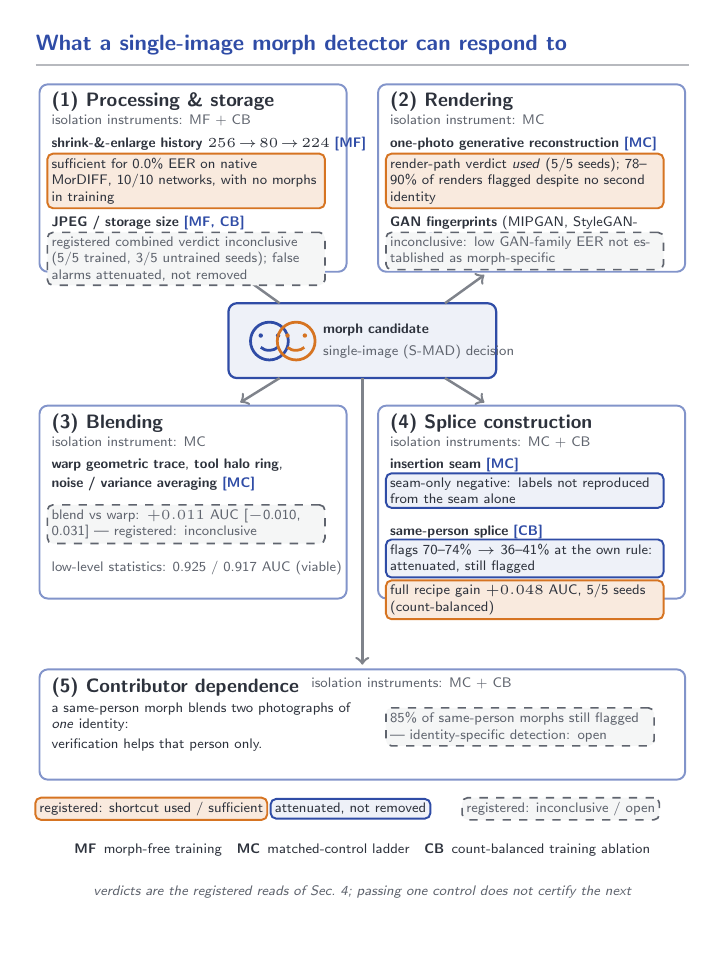
\begin{tikzpicture}[
  x=1cm,y=1cm,
  font=\sffamily,
  every node/.style={align=left, inner sep=1.5pt, outer sep=0pt},
  fline/.style={line width=1.0pt},
  hrule/.style={draw=tzGray!45, line width=0.6pt},
  boxR/.style={draw=tzBlue, fill=tzBlue!8, rounded corners=3pt, line width=0.8pt},
  fam/.style={draw=tzBlue!60, fill=white, rounded corners=3pt, line width=0.7pt},
  head/.style={anchor=west, font=\sffamily\bfseries\footnotesize, text=tzBlue},
  famHead/.style={anchor=north west, font=\sffamily\bfseries\scriptsize, text=tzDark},
  sub/.style={anchor=north west, font=\sffamily\tiny, text=tzGray},
  trait/.style={anchor=north west, font=\sffamily\tiny, text=tzDark},
  vEst/.style={draw=tzOrange, fill=tzOrange!15, rounded corners=2pt, line width=0.7pt,
               font=\sffamily\tiny, text=tzDark},
  vAtt/.style={draw=tzBlue, fill=tzBlue!8, rounded corners=2pt, line width=0.7pt,
               font=\sffamily\tiny, text=tzDark},
  vInc/.style={draw=tzGray, dashed, fill=tzGray!6, rounded corners=2pt, line width=0.6pt,
               font=\sffamily\tiny, text=tzGray},
  hint/.style={anchor=north west, font=\sffamily\tiny, text=tzGray},
  spoke/.style={->, tzGray!80, line width=0.9pt},
  qlab/.style={font=\sffamily\tiny\itshape, text=tzGray},
]
\useasboundingbox (-0.15,0.05) rectangle (8.35,11.50);

% ============================================================== header
\node[head] at (-0.1,11.28) {What a single-image morph detector can respond to};
\draw[hrule] (-0.05,11.03) -- (8.25,11.03);

% ============================================================== hub node
\draw[boxR] (2.40,7.05) rectangle (5.80,8.00);
\begin{scope}[shift={(3.02,7.52)}]
  \draw[fline, tzBlue] (-0.10,0) circle (0.24);
  \fill[tzBlue] (-0.21,0.07) circle (0.028);
  \fill[tzBlue] (0.01,0.07) circle (0.028);
  \draw[fline, tzBlue] (-0.21,-0.08) arc (215:325:0.13 and 0.09);
  \draw[fline, tzOrange] (0.24,0) circle (0.24);
  \fill[tzOrange] (0.13,0.07) circle (0.028);
  \fill[tzOrange] (0.35,0.07) circle (0.028);
  \draw[fline, tzOrange] (0.13,-0.08) arc (215:325:0.13 and 0.09);
\end{scope}
\node[anchor=west, font=\sffamily\tiny\bfseries, text=tzDark] at (3.55,7.66)
  {morph candidate};
\node[anchor=west, font=\sffamily\tiny, text=tzGray] at (3.55,7.38)
  {single-image (S-MAD) decision};

% ------------------------------------- radiating spokes: hub to trait groups
% top-left
\draw[spoke] (3.05,8.00) -- (2.55,8.36);
% top-right
\draw[spoke] (5.15,8.00) -- (5.65,8.36);
% bottom-left
\draw[spoke] (3.05,7.05) -- (2.55,6.74);
% bottom-right
\draw[spoke] (5.15,7.05) -- (5.65,6.74);
% center: down the corridor between the lower boxes to (5) contributor
\draw[spoke] (4.10,7.05) -- (4.10,3.41);

% ================================================================ 1 TL
\draw[fam] (0.00,8.40) rectangle (3.90,10.78);
\node[famHead] at (0.10,10.73) {(1) Processing \& storage};
\node[sub] at (0.10,10.44) {isolation instruments: MF + CB};
\node[trait] at (0.10,10.16)
  {\textbf{shrink-\&-enlarge history} $256\!\to\!80\!\to\!224$ {\color{tzBlue}\textbf{[MF]}}};
\node[vEst, anchor=north west, text width=3.42cm] at (0.10,9.90)
  {sufficient for 0.0\% EER on native MorDIFF, 10/10 networks, with no morphs in training};
\node[trait] at (0.10,9.16) {\textbf{JPEG / storage size} {\color{tzBlue}\textbf{[MF, CB]}}};
\node[vInc, anchor=north west, text width=3.42cm] at (0.10,8.90)
  {registered combined verdict inconclusive (5/5 trained, 3/5 untrained seeds); false alarms attenuated, not removed};

% ================================================================ 2 TR
\draw[fam] (4.30,8.40) rectangle (8.20,10.78);
\node[famHead] at (4.40,10.73) {(2) Rendering};
\node[sub] at (4.40,10.44) {isolation instrument: MC};
\node[trait] at (4.40,10.16)
  {\textbf{one-photo generative reconstruction} {\color{tzBlue}\textbf{[MC]}}};
\node[vEst, anchor=north west, text width=3.42cm] at (4.40,9.90)
  {render-path verdict \emph{used} (5/5 seeds); 78--90\% of renders flagged despite no second identity};
\node[trait, text width=3.42cm] at (4.40,9.16)
  {\textbf{GAN fingerprints} (MIPGAN, StyleGAN-style) {\color{tzBlue}\textbf{[MC]}}};
\node[vInc, anchor=north west, text width=3.42cm] at (4.40,8.90)
  {inconclusive: low GAN-family EER not established as morph-specific};

% ================================================================ 3 BL
\draw[fam] (0.00,4.25) rectangle (3.90,6.70);
\node[famHead] at (0.10,6.65) {(3) Blending};
\node[sub] at (0.10,6.36) {isolation instrument: MC};
\node[trait, text width=3.42cm] at (0.10,6.08)
  {\textbf{warp geometric trace}, \textbf{tool halo ring},\\[1pt]
   \textbf{noise / variance averaging} {\color{tzBlue}\textbf{[MC]}}};
\node[vInc, anchor=north west, text width=3.42cm] at (0.10,5.44)
  {blend vs warp: $+0.011$ AUC [$-$0.010, 0.031] --- registered: inconclusive};
\node[hint] at (0.10,4.78)
  {low-level statistics: 0.925 / 0.917 AUC (viable)};

% ================================================================ 4 BR
\draw[fam] (4.30,4.25) rectangle (8.20,6.70);
\node[famHead] at (4.40,6.65) {(4) Splice construction};
\node[sub] at (4.40,6.36) {isolation instruments: MC + CB};
\node[trait] at (4.40,6.08) {\textbf{insertion seam} {\color{tzBlue}\textbf{[MC]}}};
\node[vAtt, anchor=north west, text width=3.42cm] at (4.40,5.84)
  {seam-only negative: labels not reproduced from the seam alone};
\node[trait] at (4.40,5.24) {\textbf{same-person splice} {\color{tzBlue}\textbf{[CB]}}};
\node[vAtt, anchor=north west, text width=3.42cm] at (4.40,5.00)
  {flags 70--74\% $\to$ 36--41\% at the own rule: attenuated, still flagged};
\node[vEst, anchor=north west, text width=3.42cm] at (4.40,4.48)
  {full recipe gain $+0.048$ AUC, 5/5 seeds (count-balanced)};

% ================================================================ 5 band
\draw[fam] (0.00,1.95) rectangle (8.20,3.35);
\node[famHead] at (0.10,3.30) {(5) Contributor dependence};
\node[sub] at (3.40,3.30) {isolation instruments: MC + CB};
\node[trait, text width=3.95cm] at (0.10,2.98)
  {a same-person morph blends two photographs of \emph{one} identity:\\[1pt]
   verification helps that person only.};
\node[vInc, anchor=west, text width=3.30cm] at (4.40,2.62)
  {85\% of same-person morphs still flagged --- identity-specific detection: open};

% ============================================================== legend
\node[vEst] at (1.42,1.58) {registered: shortcut used / sufficient};
\node[vAtt] at (3.95,1.58) {attenuated, not removed};
\node[vInc] at (6.62,1.58) {registered: inconclusive / open};
\node[font=\sffamily\tiny, text=tzDark] at (4.10,1.06)
  {\textbf{MF}\, morph-free training\quad
   \textbf{MC}\, matched-control ladder\quad
   \textbf{CB}\, count-balanced training ablation};
\node[qlab] at (4.10,0.52)
  {verdicts are the registered reads of Sec.~4; passing one control does not certify the next};

\end{tikzpicture}
